\chapter{Исследовательская часть}

\section{Среда для тестирования}

Для тестирования разработанного алгоритма применялась облачная платформа Google Colab~\cite{colab}, не требующая установки ПО на локальный компьютер.

% 

\section{Тестирование классификатора}

Для классификации использовался датасет MNIST, состоящий из изображений рукописных цифр. Датасет был разделён на обучающую и тестовую выборки в пропорциях от 10\% до 90\% для обучающей выборки. Кроме того, были протестированы модели с разным количеством скрытых слоев (0, 1 и 5) для изучения влияния этой настройки на результаты классификации.

На рисунках \ref{img:learn} и \ref{img:test} приведены тепловые карты, показывающие точность тестирования моделей в зависимости от соотношения обучающей и тестовой выборок, а также от количества скрытых слоёв.

\begin{figure}
	\begin{center}
		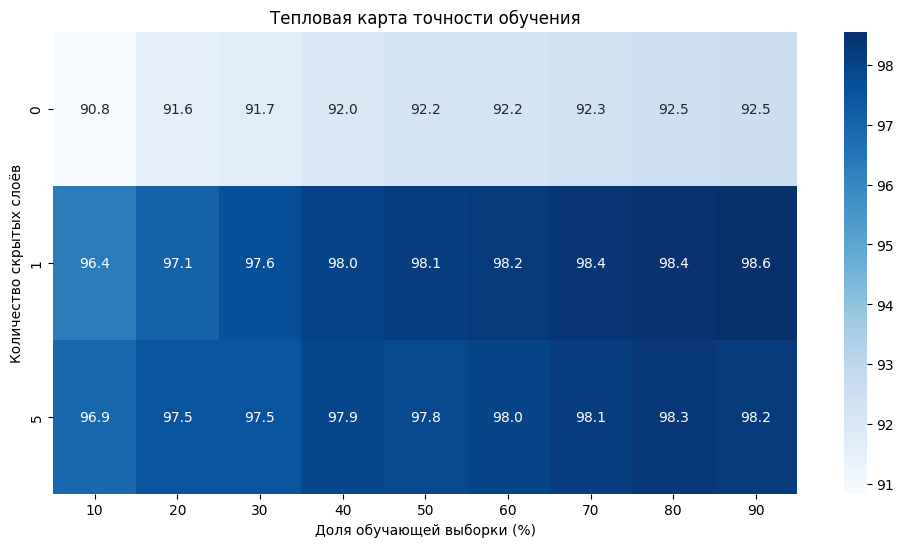
\includegraphics[width=\textwidth]{images/heatmap.png}
	\end{center}
	\caption{Тепловая карта точности обучения классификатора}
	\label{img:learn}
\end{figure}

\begin{figure}
	\begin{center}
		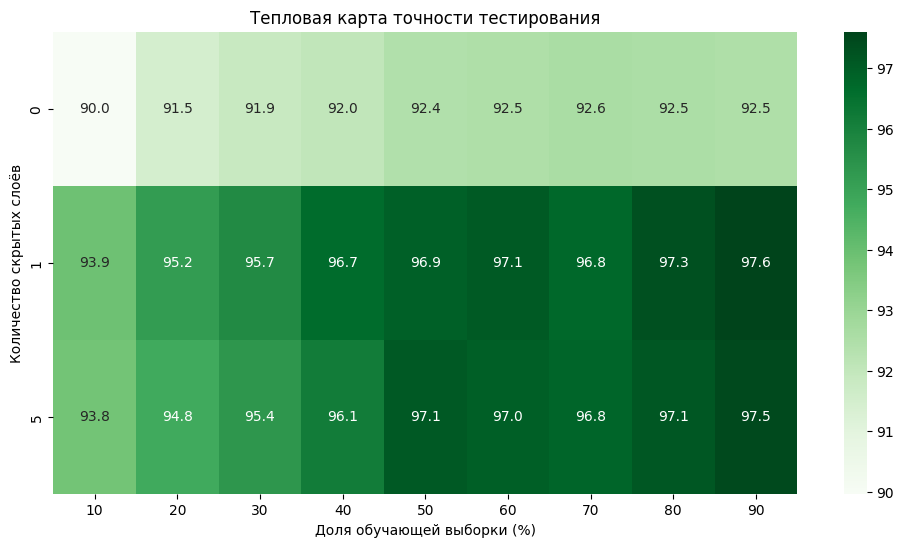
\includegraphics[width=\textwidth]{images/heatmap_test.png}
	\end{center}
	\caption{Тепловая карта точности тестирования классификатора}
	\label{img:test}
\end{figure}

Примеры состояния недообучения: соотношение обучающей и тестовой выборок 10\% к 90\% при любом количестве скрытых слоёв или 0 скрытых слоёв при любом соотношении обучающей и тестовой выборок. Примеры состояния переобучения: соотношение обучающей и тестовой выборок 70\% к 30\%, 1 или 5 скрытых слоёв.

\section{Оценка необходимого размера обучающей выборки для различных моделей}

Для каждой модели с различным количеством скрытых слоев и функцией активации была рассчитана дисперсия ошибки $\sigma^2$, а также определено минимальное количество выборки n, необходимое для достижения заданной точности. В расчётах использовались следующие параметры:
\begin{itemize}[label*=---]
	\item $\epsilon$ = 0.01 --- допустимая погрешность;
	\item $p$ = 0.95 --- доверительная вероятность.
\end{itemize}

Для вычисления необходимого размера выборки использовалась формула, основанная на втором неравенстве Чебышёва. Для различных моделей с различным количеством скрытых слоев и соотношением обучающих и тестовых данных были получены следующие результаты:
\begin{itemize}[label*=---]
	\item для соотношения обучающих данных 10\% и модели с 0 скрытыми слоями, дисперсия составила $\sigma^2$ = 0.0124, что требует минимум 261 выборку;
	\item при 1 скрытом слое дисперсия составила $\sigma^2$ = 0.0117, и необходимое количество выборок составляет 247;
	\item для модели с 5 скрытыми слоями дисперсия составила $\sigma^2$ = 0.0109, и для этого требуется 230 выборок.
\end{itemize}

Когда доля обучающих данных увеличилась до 20\%, результаты стали следующими:
\begin{itemize}[label*=---]
	\item для модели без скрытых слоев дисперсия составила $\sigma^2$ = 0.0101, что требует минимум 214 выборок;
	\item при 1 скрытом слое дисперсия была $\sigma^2$ = 0.0098, что потребовало 208 выборок;
	\item для модели с 5 скрытыми слоями дисперсия составила $\sigma^2$ = 0.0094, и необходимое количество выборок составило 200..
\end{itemize}

При доле обучающих данных 90\%, результаты следующие:
\begin{itemize}[label*=---]
	\item для модели с 0 скрытыми слоями дисперсия составила $\sigma^2$ = 0.0051, что требует минимум 109 выборок;
	\item при 1 скрытом слое дисперсия составила $\sigma^2$ = 0.0050, и необходимое количество выборок составило 107;
	\item для модели с 5 скрытыми слоями дисперсия составила $\sigma^2$ = 0.0048, что требует 103 выборок.
\end{itemize}

\section*{Вывод}

Время выполнения программы в среде Google Colab составило приблизительно 10 минут. Данный эксперимент был проведён с использованием стандартных вычислительных ресурсов, включая графические ускорители, повышающие производительность обучения.

Точность модели зависит от соотношения обучающих и тестовых выборок. Оптимальное соотношение составляет 90\% обучающих данных и 10\% тестовых. Именно при таком соотношении при использовании одного скрытого слоя достигается наивысшая точность обучения (98.6\%) и тестирования (97.6\%).

Увеличение количества скрытых слоёв в модели повышает точность на обеих выборках, однако слишком большое количество слоев может привести к переобучению. Оптимальное количество скрытых слоев для данной задачи --- 1.

Применение неравенства Чебышева позволяет оценить надежность модели и ее стабильность в процессе обучения.

\clearpage
